\chapter{INTRODUCTION}
% (20% of Proposal Length)
\pagenumbering{arabic}

% Introduction: (20\% of Report Length)


\section{Introduction}
LabXplorerX is revolutionizing science education by providing an innovative interactive learning platform designed to transcend traditional learning methods. Specifically tailored for students and educators in STEM fields, LabXplorerX aims to bridge gaps in practical science education by offering interactive simulations across diverse disciplines. This cutting-edge platform serves as a dedicated arena where scientific concepts can be engaged with deeply, virtual simulations can be conducted, can be visualized, and seamless collaboration can be achieved within the academics.LabXplorerX addresses critical gaps in science education by providing a dedicated platform specifically designed for simulations tailored to students in grades 7, 8, and 9. Unlike general educational platforms that lack interactive simulation components, LabXplorerX offers specialized modules such as Basic Electronics Simulations, Basic Chemistry Simulations, Basic Astronomy Simulations, and a Basic Online Coding Environment with animations. This targeted approach allows students to gain hands-on experience and apply theoretical knowledge in practical settings, thereby enhancing their understanding and retention of scientific concepts.


\section{Problem Statement }
LabXplorerX addresses critical gaps in science education by providing a dedicated platform specifically designed for virtual laboratory simulations for students of grades 7, 8, and 9. Unlike general educational platforms that lack interactive simulation components, LabXplorerX offers tailored modules such as Basic Electronics Simulations, Basic Chemistry Simulations, Basic Astronomy Simulations, and a Basic Online Coding Environment with animations. This specialized approach enables students to gain hands-on experience and apply theoretical knowledge in practical settings, enhancing their understanding and retention of scientific concepts.
\section{Objectives}
\begin{itemize}
    \item Create an interactive learning platform for students from Grade 7,8,9 that enhances STEM education through inter-active simulations aweb various disciplines.

\end{itemize}
\section{Scope}
% Scope and limitation

\begin{itemize}
    \item The platform should provide a virtual space for students and educators to conduct interactive simulations and promote simulating learning.
    \item LabXplorerX facilitates collaborative learning through comments, enabling students to share insights and ask questions.
    \item The platform should be user-friendly and accessible, making it easy for students to engage in.
    \item LabXplorerX includes learning capsules where students can gain in-depth knowledge and understanding of various scientific concepts.
\end{itemize}
\section{Limitation}
% Scope and limitation

\begin{itemize} 
    \item The creation of simulations is restricted to developers, as users and super users do not have the capability to create new simulations. 
    \item The platform lacks mobile responsiveness for simulations, which limits accessibility and usability of simulations on mobile devices. 
\end{itemize}

\section{Development methodology}
FFor the development of LabXplorerX, the Rapid Application Development (RAD) methodology is employed. This approach emphasizes iterative development and continuous user feedback rather than rigid planning. By engaging a diverse range of stakeholders, including friends, family, and esteemed faculty members from the Department of Computer Application, valuable insights on usability and functionality are gathered. This engagement allows for practical feedback from potential end-users and expert advice on educational and technological standards. As a result, LabXplorerX evolves in response to real user needs and academic requirements, ensuring the development of a more effective and user-centric platform for science education.

This iterative process ensures that LabXplorerX evolves in response to real user needs and academic requirements, resulting in a more effective and user-centric platform for science education.
\section{Report Organisation}
The material in this project report is organised into Six chapters. After this introductory chapter introduces the problem topic this project tries to address, chapter 2 contains the literature review of vital and relevant publications, pointing toward a notable project related infromations. Chapter 3 describes the Designs and Analysis of the System for the implementation of this project and models and methods. Chapter 4 provides an overview of Implementation tools, modules used and testing performed in certain unit. Chapter 5 Lesson Learn with outcomes including future recommendations. After Main Report contains have Appendix A that contains Gantt Chart and Supervisor Consultation form. Last one contains Referneces.
\begin{figure}[H]
    \centering
     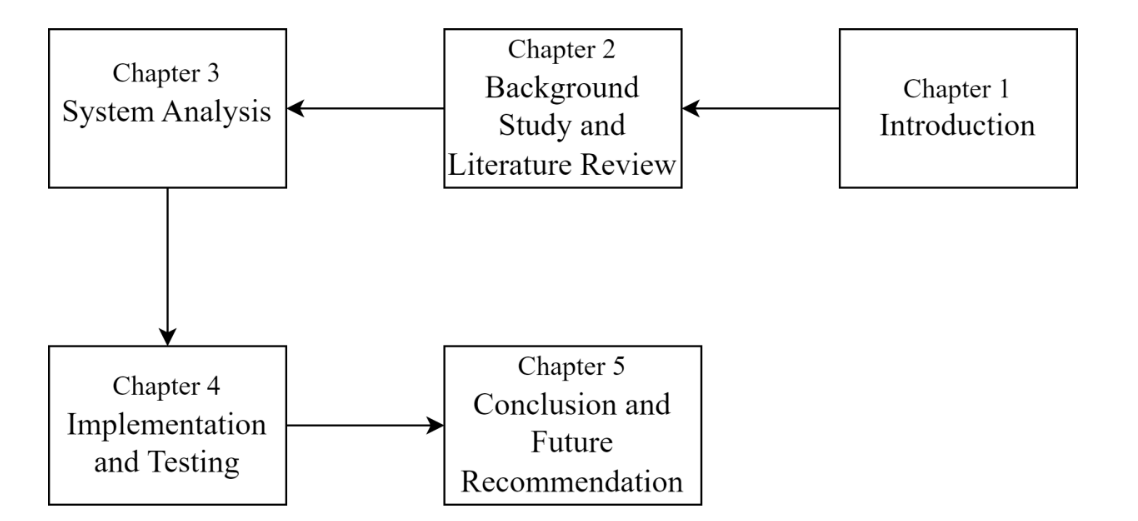
\includegraphics[height = 6cm]{Diagrams/organization.png}
     \caption{Report Organisation}
 \end{figure}